\begin{figure}[H]
    \centering
    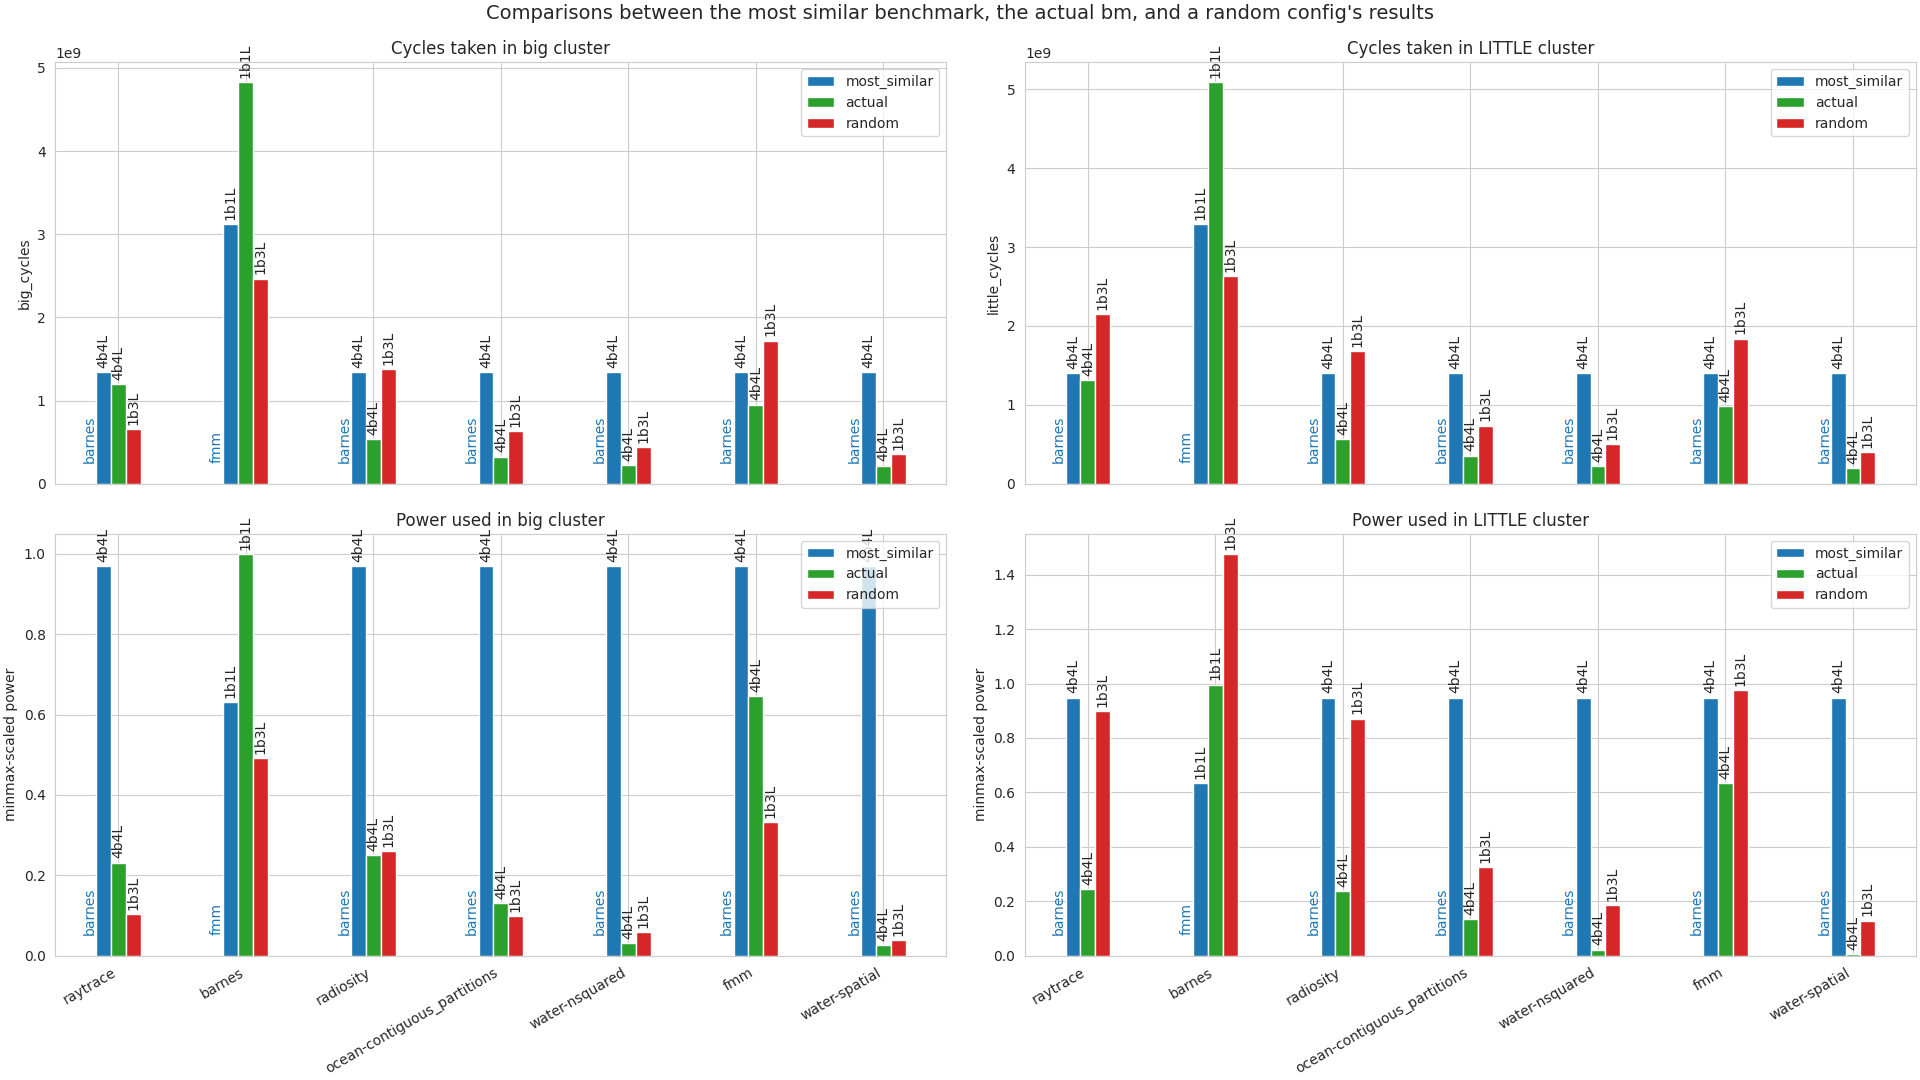
\includegraphics[height=0.4\textheight]{pred-plots/stock-2b2L-3b1L/rand-1b3L.png}
    \caption{Performance comparisons using 2b2L+3b1L as stock, 1b3L as baseline}
\end{figure}

\begin{figure}[H]
    \centering
    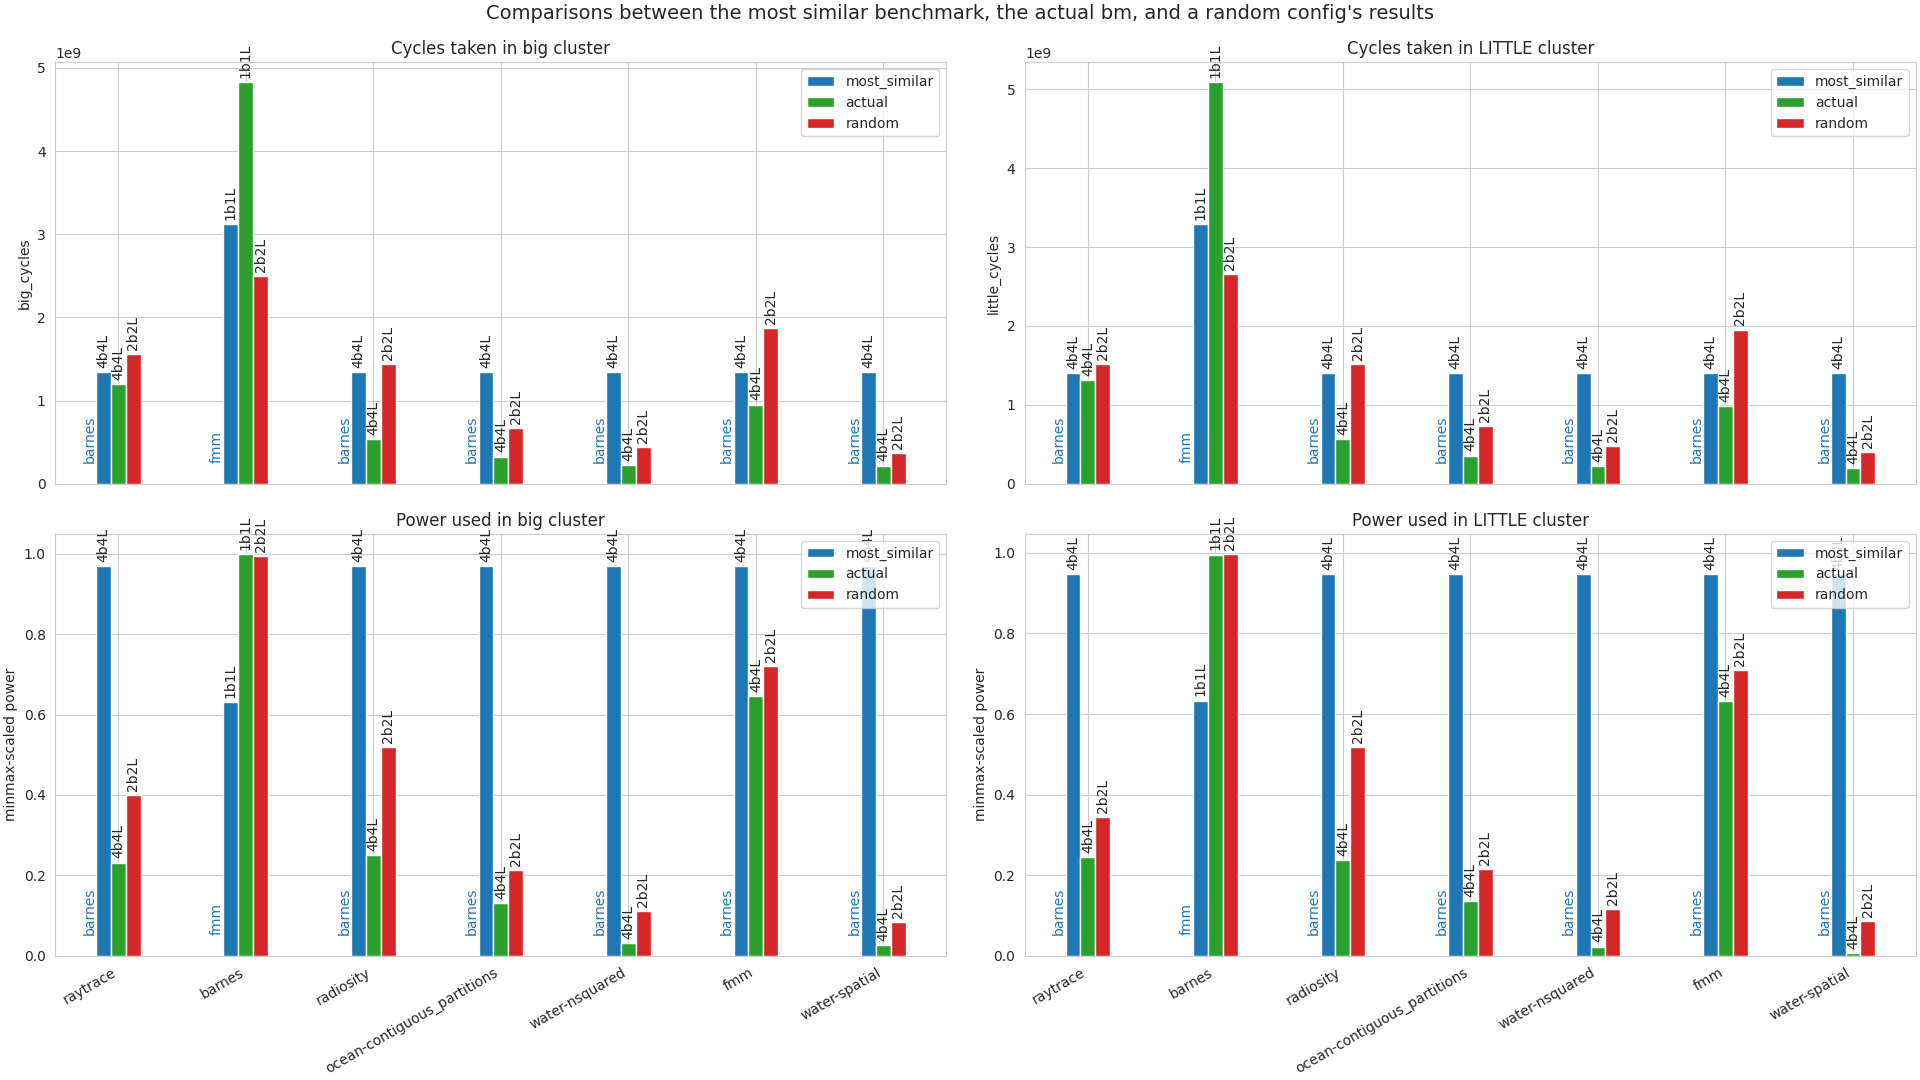
\includegraphics[height=0.4\textheight]{pred-plots/stock-2b2L-4b4L/rand-2b2L.png}
    \caption{Performance comparisons using 2b2L+4b4L as stock, 2b2L as baseline}
\end{figure}

\begin{figure}[H]
    \centering
    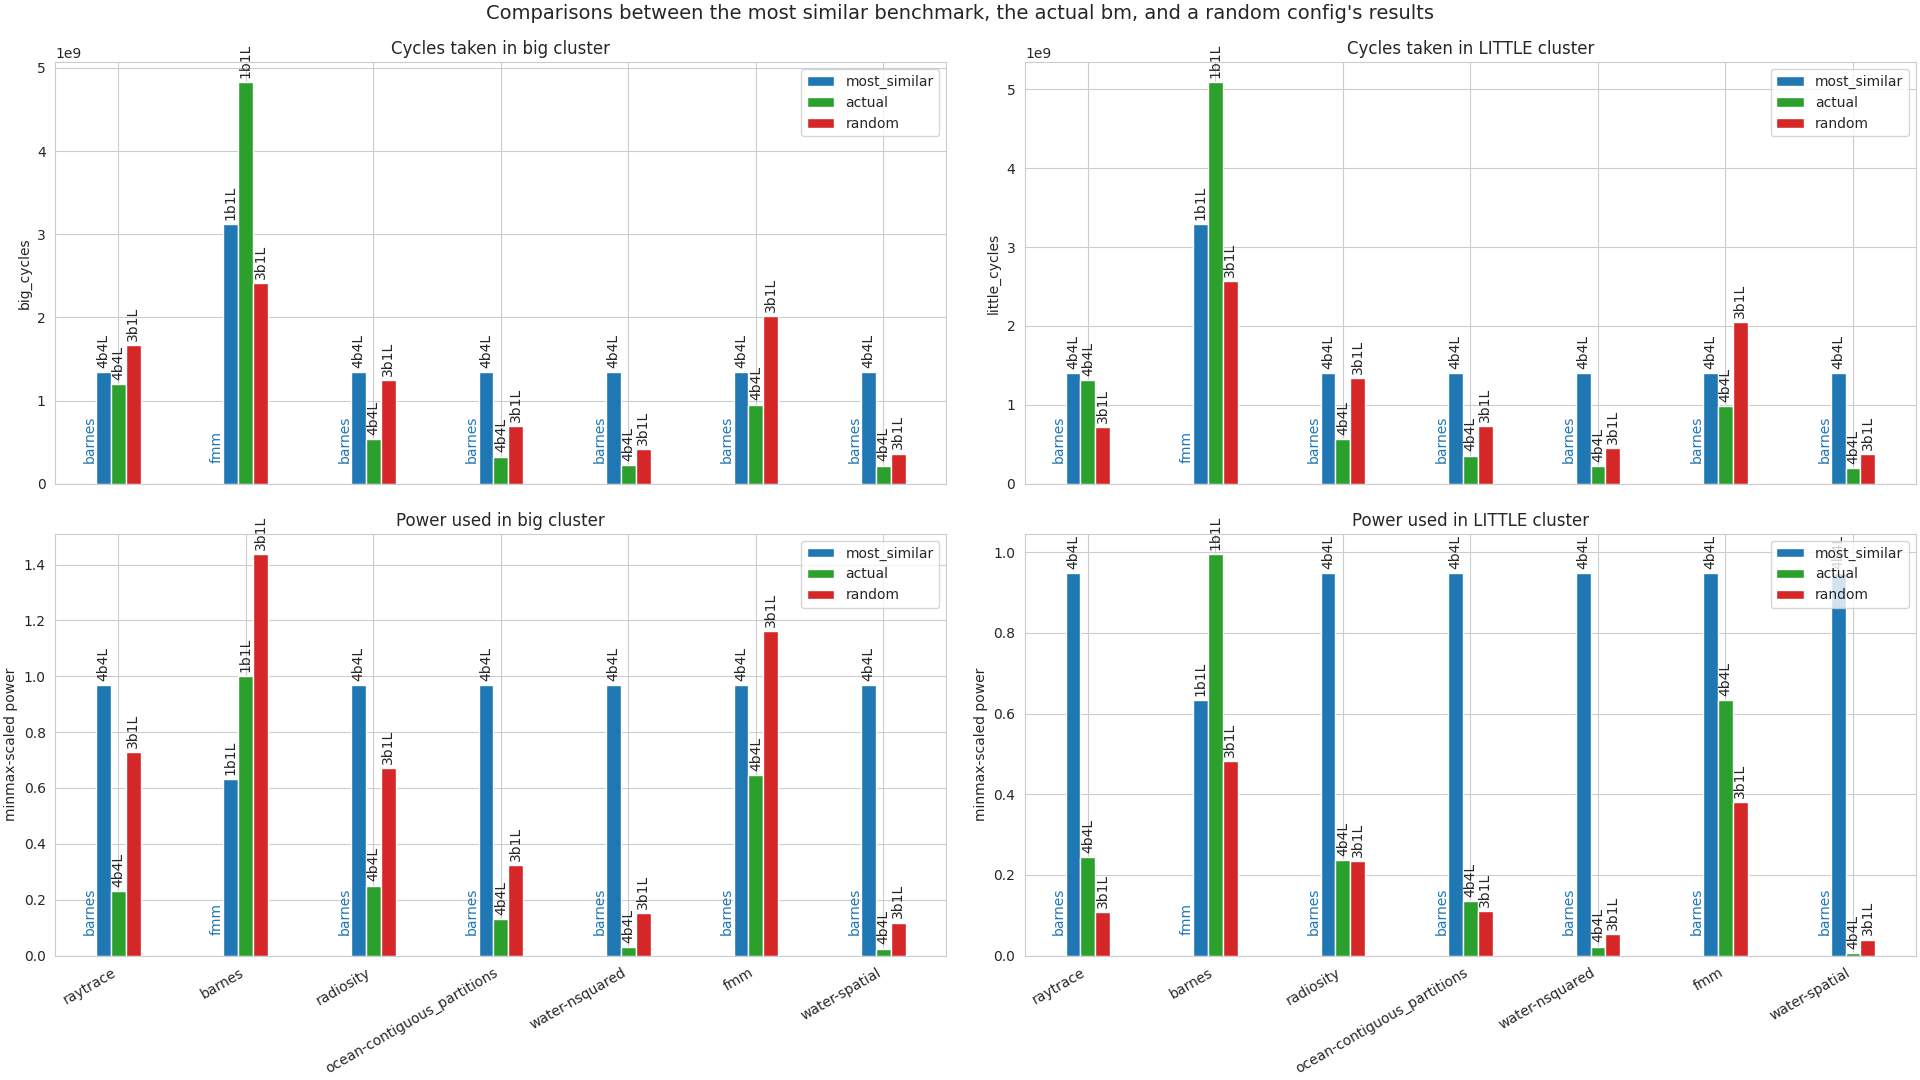
\includegraphics[height=0.4\textheight]{pred-plots/stock-3b1L-1b3L/rand-3b1L.png}
    \caption{Performance comparisons using 3b1L+1b3L as stock, 3b1L as baseline}
\end{figure}
